\section{Бинаризация изображений}

Бинаризация изображения выполняется по следующему алгоритму:
\begin{equation}
    I_{new}(x, y) = \begin{cases}
        0, & I(x, y) \le t,\\
        1, & I(x, y) > t,
    \end{cases}
\end{equation}
где $t$ -- порог бинаризации. 

Или, в случае двойного порога: 
\begin{equation}
    I_{new}(x, y) = \begin{cases}
        0, & I(x, y) \le t_1,\\
        1, & t_1 < I(x, y) \le t_2, \\
        0, & I(x, y) > t_2
     \end{cases}
\end{equation}
где $t_1$, $t_2$ -- верхний и нижний порог бинаризации соответственно. 


\FloatBarrier
\subsection{Бинаризация по среднему значению}
В данном случае, в качестве порога выберем среднее значение яркости пикселей, вычисляемое по формуле
\begin{equation}
    t = \frac{I_{max} - I_{min}}{2}
\end{equation}
где $I_{max}$ -- максимальное значение яркости пикселей, $I_{min}$ -- минимальное значение яркости пикселей.

Полученное в результате бинаризации изображение представлено на рисунках \ref{img:binarization_mean} и~\ref{img:binarization_mean_inv}. Значение порога бинаризации при этом оказалось равным 127.
\begin{figure}[ht!]
    \centering
    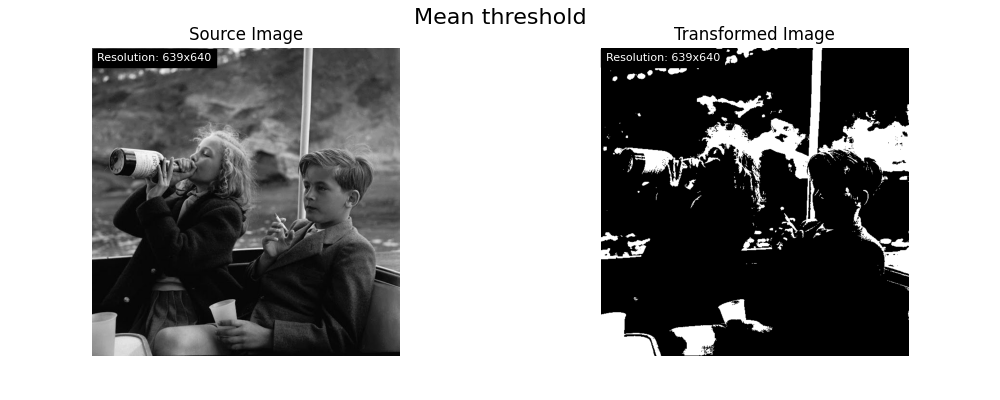
\includegraphics[width=\textwidth]{../results/Mean threshold.png}
    \caption{Результат бинаризации по среднему значению}
    \label{img:binarization_mean}
\end{figure}

\begin{figure}[ht!]
    \centering
    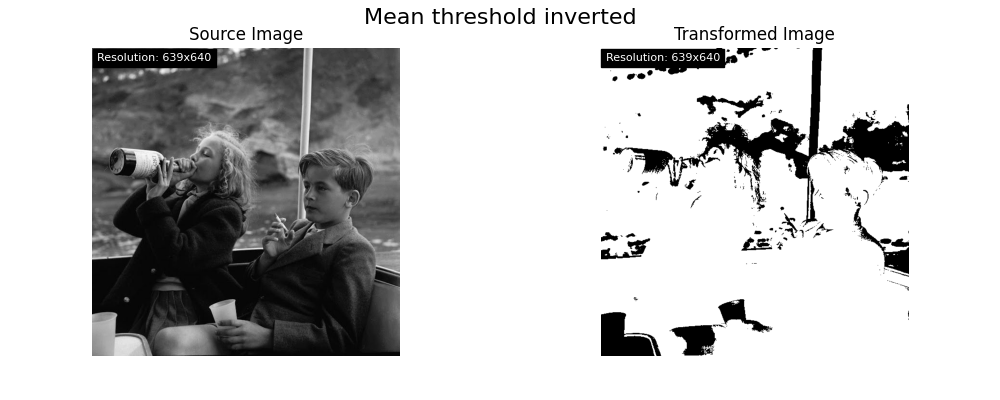
\includegraphics[width=\textwidth]{../results/Mean threshold inverted.png}
    \caption{Результат бинаризации по среднему значению (инвертированная)}
    \label{img:binarization_mean_inv}
\end{figure}

Видим, что, как и ожидалось, в случае с бинаризацией по нижнему порогу, все пиксели темнее среднего значения стали черными, а светлее -- белыми. В случае бинаризации по верхнему порогу, наоборот, все пиксели светлее среднего значения стали черными, а темнее -- белыми.


\FloatBarrier
\subsection{Бинаризация по модулю градиента}
В данном случае значение порога бинаризации $t$ выбирается по следующей формуле:
\begin{equation}
    t = \frac{\sum_{x = 0}^{X - 1}\sum_{y = 0}^{Y - 1}I(x, y)G(x, y)}{\sum_{x = 0}^{X - 1}\sum_{y = 0}^{Y - 1}G(x, y)}
\end{equation} 
где $G(x, y)$ -- модуль градиента изображения, вычисляемый по формуле: 
\begin{equation}
    G(x, y) = \max{|I(x + 1, y) - I(x - 1, y)|, |I(x, y + 1) - I(x, y - 1)|}
\end{equation}
Исходный код для вычисления порога бинаризации на основе градиента представлен в листинге \ref{lst:calc_gradient_threshold}.

Полученное в результате бинаризации изображение представлено на рисунке \ref{img:binarization_gradient} и~\ref{img:binarization_gradient_inv}. Значение порога бинаризации при этом оказалось равным 196.
\begin{figure}[ht!]
    \centering
    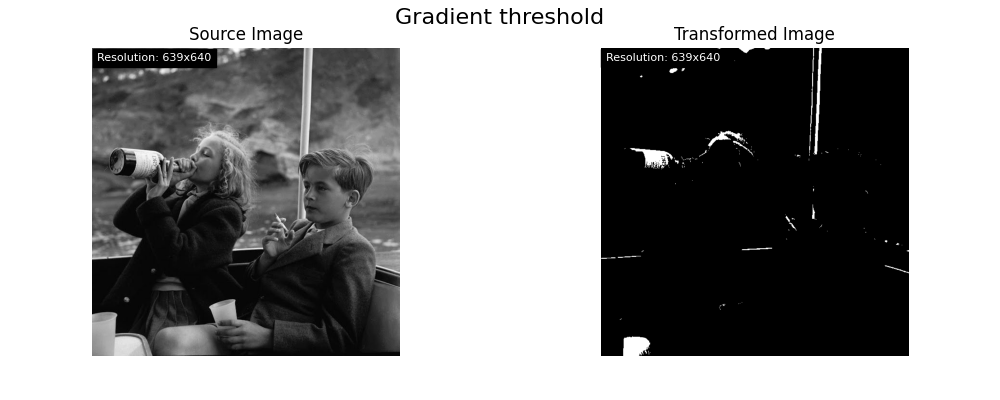
\includegraphics[width=\textwidth]{../results/Gradient threshold.png}
    \caption{Результат бинаризации по модулю градиента}
    \label{img:binarization_gradient}
\end{figure}

\begin{figure}[ht!]
    \centering
    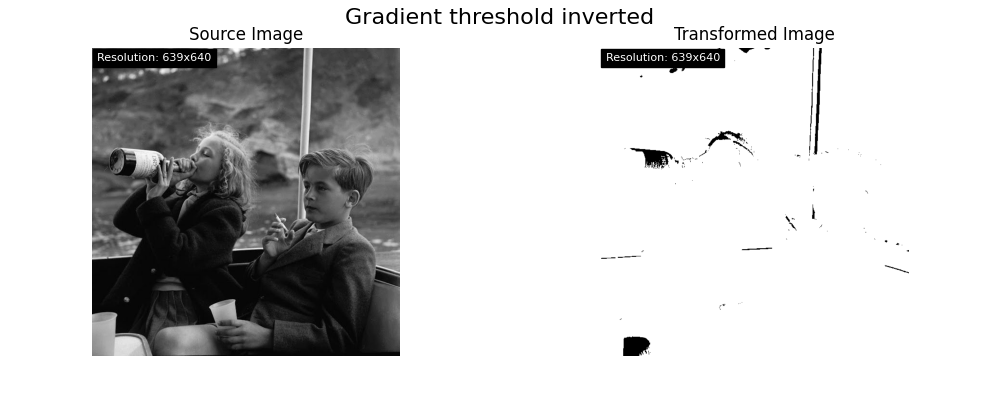
\includegraphics[width=\textwidth]{../results/Gradient threshold inverted.png}
    \caption{Результат бинаризации по модулю градиента (инвертированная)}
    \label{img:binarization_gradient_inv}
\end{figure}

Видим, что при увеличении значения порога бинаризации, увеличивается количество черных пикселей на изображении.

Метод вычисления порога бинаризации на основе градиента показал себя на данном изображении не лучшим образом. Оно практически все стало черным. 

\FloatBarrier
\subsection{Бинаризация по методу Отсу}

В методе Отсу порог бинаризации выбирается таким образом, чтобы минимизировать внутриклассовую дисперсию и максимизировать межклассовую дисперсию.
В Python есть реализация метода Отсу в библиотеке OpenCV. Полученное в результате бинаризации изображение представлено на рисунках \ref{img:otsu_threshold} и~\ref{img:otsu_threshold_inv}.

В данном случае значение порога бинаризации $t$ оказалось равным 78.
\begin{figure}[ht!]
    \centering
    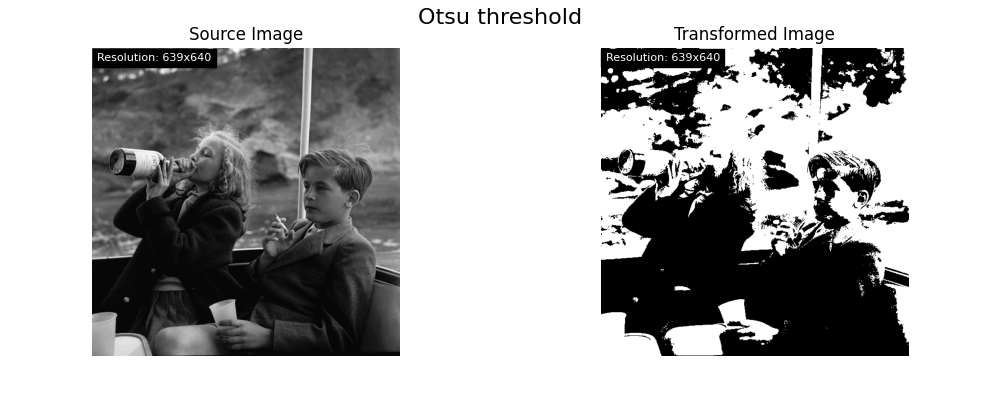
\includegraphics[width=\textwidth]{../results/Otsu threshold.png}
    \caption{Результат бинаризации по принципу Отсу}
    \label{img:otsu_threshold}
\end{figure}

\begin{figure}[ht!]
    \centering
    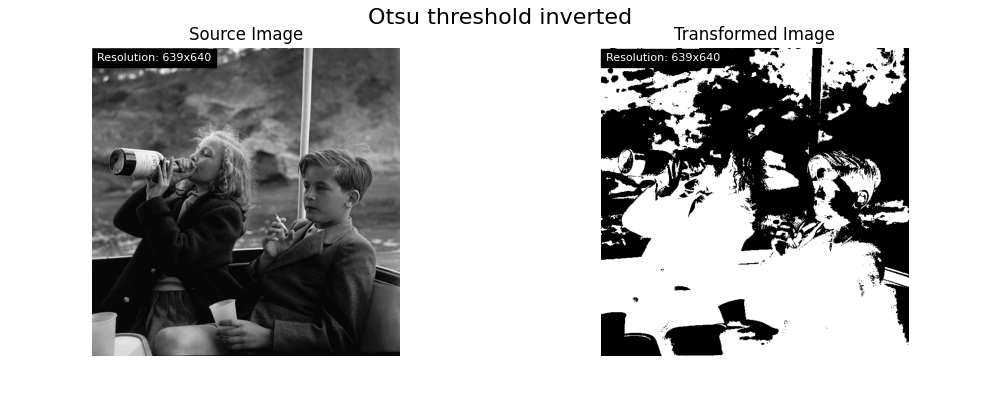
\includegraphics[width=\textwidth]{../results/Otsu threshold inverted.png}
    \caption{Результат бинаризации по принципу Отсу (инвертированная)}
    \label{img:otsu_threshold_inv}
\end{figure}

Бинаризация на основе алгоритма Отсу хорошо сработала в данном случае. На изображении, хоть оно и является черно-белым, хорошо различимы объекты.

\FloatBarrier
\subsection{Адаптивная бинаризации}

Адаптивная бинаризация позволяет учитывать различные особенности изображения, такие как освещенность, контрастность и т.д. В данной работе рассмотрены два метода адаптивной бинаризации: на основе среднего и на основе функции Гаусса.

\subsubsection{Адаптивная бинаризация на основе среднего}

\begin{figure}[ht!]
    \centering
    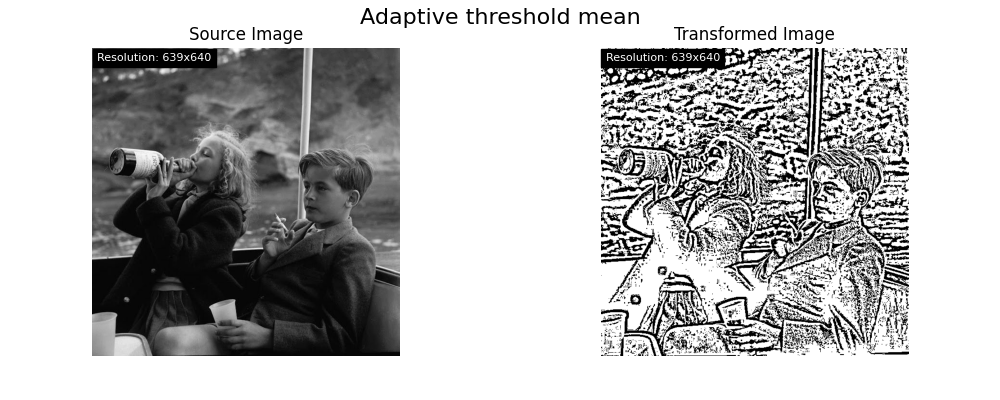
\includegraphics[width=\textwidth]{../results/Adaptive threshold mean.png}
    \caption{Результат адаптивной бинаризации на основе среднего}
    \label{img:adaptive_mean}
\end{figure}

\begin{figure}[ht!]
    \centering
    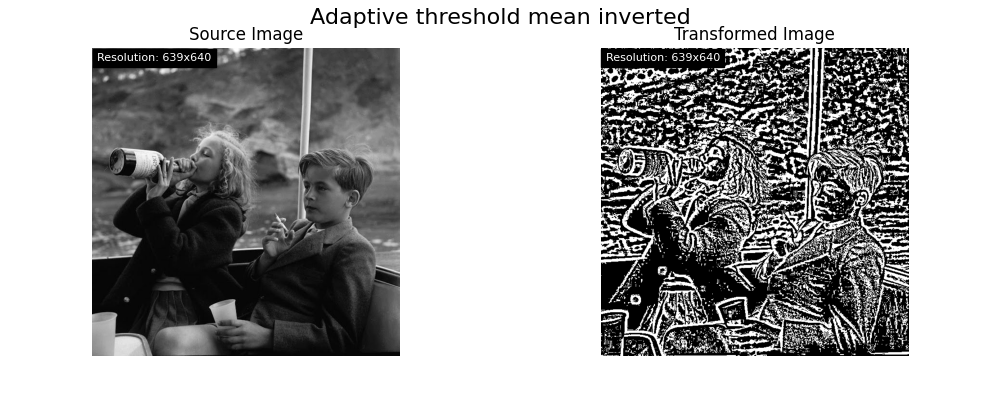
\includegraphics[width=\textwidth]{../results/Adaptive threshold mean inverted.png}
    \caption{Результат адаптивной бинаризации на основе среднего (инвертированная)}
    \label{img:adaptive_mean_inv}
\end{figure}

Этот метод бинаризации отличается от всех ранее рассмотренных. Субъективно, он больше похож на алгоритм выделения контуров, чем на бинаризацию. 
\FloatBarrier
\subsubsection{Адаптивная бинаризация на основе Функции Гаусса}

\begin{figure}[ht!]
    \centering
    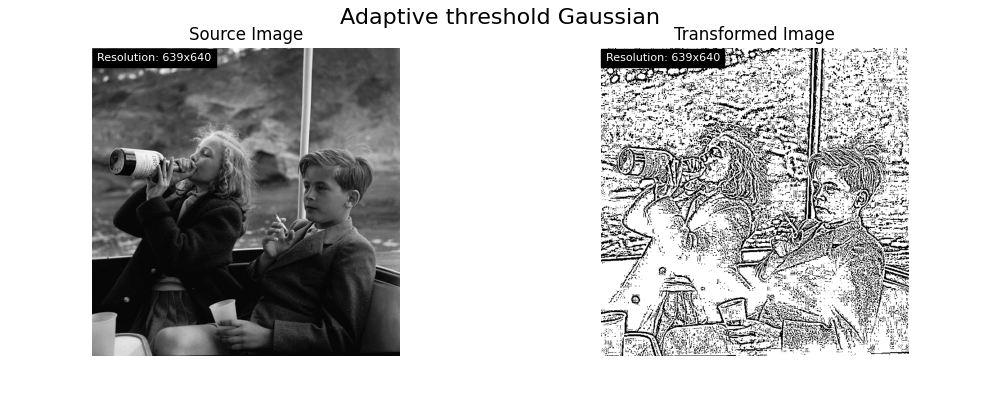
\includegraphics[width=\textwidth]{../results/Adaptive threshold Gaussian.png}
    \caption{Результат адаптивной бинаризации на основе функции Гаусса}
    \label{img:adaptive_gaussian}
\end{figure}

\FloatBarrier
\begin{figure}[ht!]
    \centering
    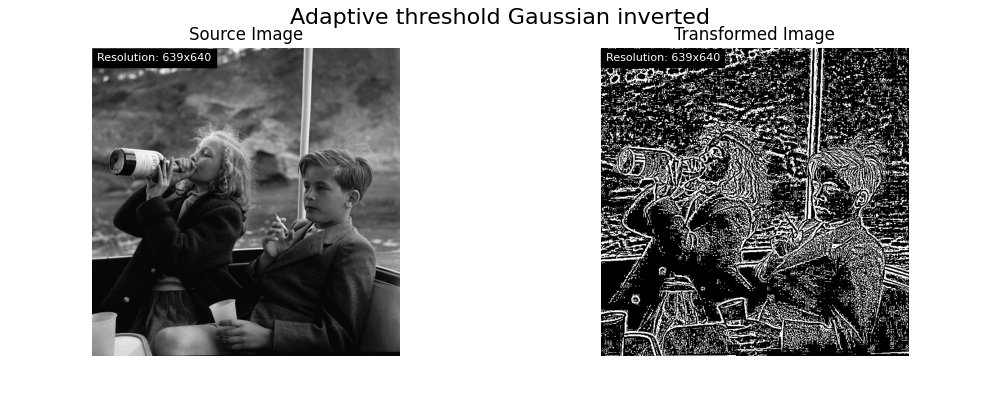
\includegraphics[width=\textwidth]{../results/Adaptive threshold Gaussian inverted.png}
    \caption{Результат адаптивной бинаризации на основе функции Гаусса (инвертированная)}
    \label{img:adaptive_gaussian_inv}
\end{figure}

Данный способ бинаризации очень схож с прошлым, на основе среднего. Однако, он более гладкий и мягкий.

